% File for libamtrack manual
% Copyright 2006, 2010 Steffen Greilich / the libamtrack team
% This file is part of the libAmTrack project (libamtrack.dkfz.org).

\chapter{\la{} methods}

\section{Introduction}
'Methods' are the top-level routines in \la{}. From the physical parameters describing a HCP field they compute the predicted RE or RBE. In order to do so, the user has to both chose 
\begin{itemize}
\item{method independent settings, such as the radiation field, RDD, ER, gamma model and}
\item{method specific setting, e.g. the binning width to be used.}
\end{itemize}

Methods are implemented in the \texttt{Amtrack.c} and make use of all other subordinate routines. At the moment, four methods are available, Tab. \ref{tbl:Methods} gives an overview. All 	methods apply to slice of a homogenous detector being infinitesimally small in $z$ direction\footnote{Or a slice of the detector with finite size in $z$ but with crucial parameters, such as LET, fluence etc. not changing significantly over $\Delta z$}, i.e. in direction of the beam. The latter is supposed to be perfectly parallel and homogenous in fluence with respect to $x$ and $y$ (Fig. \ref{fig:Coordinates}. 

\begin{figure*}
	\centering
		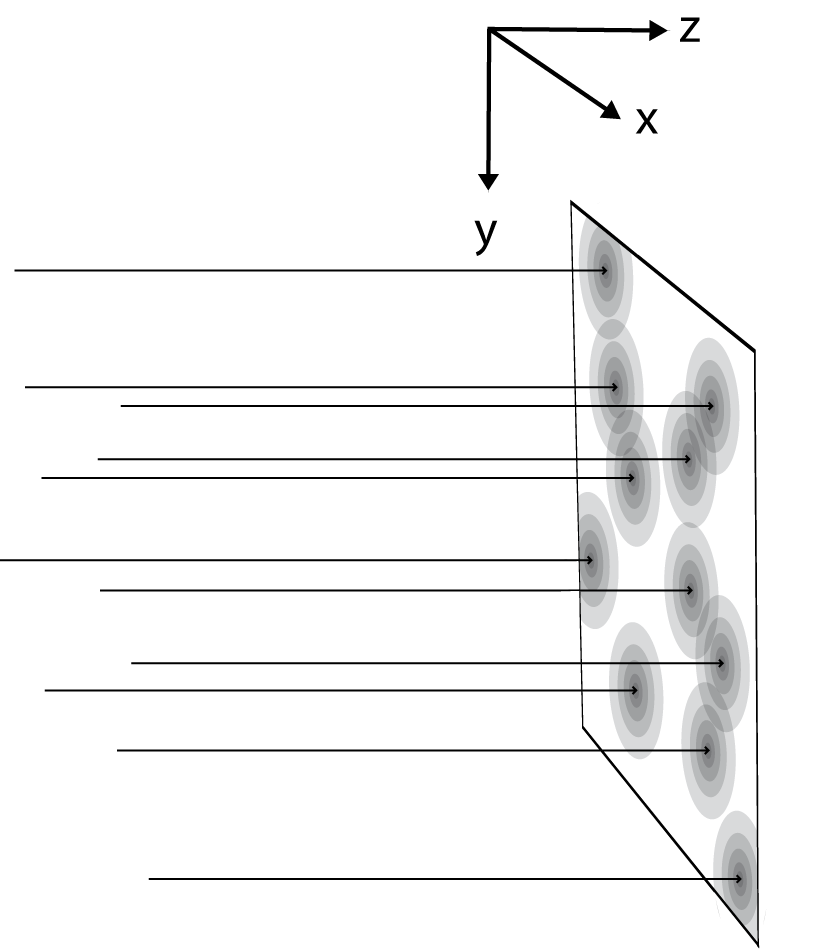
\includegraphics[bb=0 0 839 952,width=0.5\textwidth]{pictures/CoordinatesMethods.png}
	\caption{Coordinate definition in \la{}}
	\label{fig:Coordinates}
\end{figure*}

All methods share the following input parameters:\\
\begin{tabular}{p{0.25\textwidth} p{0.75\textwidth}}
\texttt{n} & number of components in mixed field (long integer) \\
\texttt{E\_MeV\_u[]} & the kinetic energy per nucleon for each component (array of double, size \texttt{n}) \\
\texttt{particle\_no[]} & the particle id number for each component, see ref. for more details (array of long, size \texttt{n}) \\
\texttt{fluence\_cm2[]} & the fluence (in cm$^{-2}$) or the dose (in Gy), if negative, for each component (array of double, size \texttt{n}) \\
\texttt{material\_no} & the material id number (long integer) \\
\texttt{rdd\_model} & the radial dose distribution id number, see \ref{chap:RDDs} for details (long) \\
\texttt{rdd\_parameters[]} & parameters for the given RDD, see \ref{chap:RDDs} for details (array of long, size depending on RDD model) \\
\texttt{er\_model} & the electron range id number, see \ref{chap:ERs} for details (long) \\
\texttt{gamma\_model} & the photon response id number, see \ref{chap:GRs} for details (long) \\
\texttt{gamma\_parameters[]} & parameters for the given RDD, see \ref{chap:GRs} for details (array of long, size depending on GR model) \\
\end{tabular}\\

All methods need in addition an array to return their results:\\
\begin{tabular}{p{0.25\textwidth} p{0.75\textwidth}}
\texttt{results[]} & the particle id number for each component (array of long, size 10) \\
\end{tabular}

\begin{table}
\label{tbl:Methods}
\begin{tabular}{m{0.25\textwidth}m{0.60\textwidth}m{0.15\textwidth}}

\hline
\textbf{Name} & \textbf{Description} & \textbf{Reference} \\
\hline

\begin{center}Ion-Gamma-Kill (IGK)\end{center}&
\footnotesize{Get activation cross-section by fusing photon response (activation probability) and RDD, get particle response by cross-section and fluence (ion-kill, intratrack action), for multi-hit systems and lower LET consider also intertrack action (gamma kill).}&
\begin{center}\cite{Waligorski_and_Katz_1980}\end{center}\\

\begin{center}Grid summation (GSM)\end{center}&
\footnotesize{,,Throw'' of particle tracks on a Cartesian grid for local dose, apply photon response for local response, then average response.}&
\begin{center}\cite{Geiss_et_al_1997}\end{center}\\

\begin{center}Compound Poisson processes using successive convolution (CPP-SC)\end{center}&
\footnotesize{Derive local dose frequency distribution analytically from RDD for single particle case, assume �none or one-impact situation for low fluence, convolute resulting distribution with itself until desired high fluence / dose is reached, apply photon response.}&
\begin{center}\cite{Greilich_et_al_CPPSC}\end{center}\\

\begin{center}Compound Poisson processes using statistical sampling (CPP-SS, SPISS)\end{center}&
\footnotesize{Derive local dose frequency distribution analytically from RDD for single particle case � as for CPPSC. But then use statistical sampling to add single impact doses according to relative fluences in the particle field.} &
\begin{center}\cite{Greilich_et_al_CPPSC}\end{center}\\

\hline
\end{tabular}
\caption{Methods implemented in \la{}.}
\end{table}


\section{The grid summation method (GSL)}
This is the most straight-forward approach: particles are sampled according to their relative fluence and local doses $d(x,y)$ --- and therefore local response $s(x,y)=S_X(d(x,y))$ --- are computed on a Cartesian grid ('checkerboard') by attributing the corresponding $d_{E,T}(r)$ to the sampled particle (FIGURE?). The detector is thought to be homogenous, perpendicular to the beam in $(x,y)$, and of negligible thickness $\Delta z$. The relative efficiency $\eta$ can then be estimated by averaging the local response $s$ over all grid elements:
\begin{equation}\label{eq:eta}
	\eta(\phi(E, T))=\frac{S_{HCP}}{S_X(D)}=\frac{\left\langle s\right\rangle}{S_X(\left\langle d\right\rangle)}
\end{equation}

Although conceptually straightforward, GSM can be very time-consuming, esp. in the case of higher fluences and particle energies (e.g. $E_{\mbox{proton}} >$ 20 MeV) with many contributions to a single voxel. Furthermore, the procedure has to be repeated many times in order to converge --- or a large detector grid has to be simulated. 


\section{The compount Poisson process methods (CPP)}

To overcome the limitations of GSM calculating the local dose distibution as a spatial deposition pattern $d(x,y)$, we consider a representative point $P$ (FIGURE?). The cumulative distribution function $F(d)$ of local dose $d$ in $P$ depends on the macroscopic fluence $\phi$ (and dose $D$, resp.) and the microscopic pattern around a track as expressed by $d(r)$. Then, one can state:
\begin{itemize}
	\item {$r_{max}$ is the maximum delta electron range in the field, so $P$ is only influenced by tracks within a circle $C$ of radius $r_{max}$ around $P$ (\mbox{FIGURE?}).}
	\item {All tracks in $C$ are contributing to $d$ and their number $n$ is Poisson distributed with mean $\mu=\phi\cdot\pi r_{max}^2$.}
	\item {Let $F_n$ be the cumulative distribution function of the local dose in the case of exactly $n$ tracks. For a single track traversing $C$, we readily have the cumulative single impact distribution
		\begin{equation}\label{eq:singletrack}
			F_1(d)=1-\frac{R(d)^2}{r_{max}^2},
		\end{equation}
		with $R(d)=D^{-1}(r)$ (\mbox{FIGURE?}).}
	\item {In the case of $n$ tracks in $C$, $d$ is the sum of $n$ independent and identically distributed single track doses, so $F_n$ can be expressed as the $n$-fold convolution of $F_1$:
		\begin{equation}\label{eq:ntracks}
			F_n=\underbrace{F_1*\ldots*F_1}_{\mbox{$n$ times}}
		\end{equation}
	}
	\item {As $n$ is Poisson distributed, $F$ is the distribution function of a compound Poisson process:
		\begin{equation}
			F(d)=e^{-\mu}\sum^{\infty}_{i=1}{\frac{\mu^i}{i!}F_i(d)}
		\end{equation}
	}
	\item {The derivative $f(d)$ of $F(d)$ can then be eventually used to compute the macroscopic HCP detector response as the expected local response $\left\langle s\right\rangle$:
		\begin{equation}
		  \langle s \rangle= \int_0^{\max(d)} S_X(d) f(d)\, \mathrm{d}d,
		\end{equation}
		and used in Eq. (\ref{eq:eta}) to get the $\eta$. A similar procedure for $\left\langle d\right\rangle$ provides a quality check as it has to meet $D$.
	}
\end{itemize}
This description enables $F$ to be determined from the explicitly given distribution function $F_1$ in the case of monoenergetic particle fields. It can easily be extended to mixed particle fields by using the adjusted $F_1$ from Eq.(\ref{eq:multitrack}) in Eq.(\ref{eq:ntracks}) with $p_{E,T}$ being the relative fluence and $R_{E,T}$ the inverse radial dose distribution for the composing particles
\begin{equation}\label{eq:multitrack}
  F_1(d)=1-\sum_{E,T}p_{E,T}\cdot\frac{R_{E,T}(d)^2}{\hat{r}_{max}^2},
\end{equation}
where $\hat{r}_{max}=max(r_{max}(E,T))$.

It should be stressed that the presented approach is in no way limited to handle extended targets despite the point nature of $P$ as the averaging across the target is already contained in $D(r)$ (for the difference between point and extended target distributions, see \cite{Katz_et_al_1972, Edmund_et_al_2007}). While the computation of detector response from the local dose distribution $F(d)$ is trivial, the numerical calculation of $F(d)$ itself can, however, be cumbersome. 



\subsection{Computation using statistical sampling (CPP-SS)}
One way to approximate $F(d)$ is the following:


The implementation of this approach in \la{} is named SPISS, which is explained below.



\subsection{Accelerated computation using successive convolution (CPP-SC)}
An approximation method for the rapid computation of compound Poisson processes was introduced by Kellerer \cite{Kellerer_1985}. It makes use of the fact that the distribution $f(d;\mu)$ can be obtained by a convolution operation:
	\begin{equation}
		f(d;\mu)=\int_{0}^{d}{f(d-t;\mu/2)\cdot f(t;\mu/2) dt}
	\end{equation}
One can chose a $\mu_{start}<<1$ with $\mu=2^m\cdot\mu_{start}$ so that multiple events can be neglected and therefore $f(d;\mu_{start})$ consists, in good approximation, of two components only, namely the probability of no track in $C$ ($d=0$) 
	\begin{equation}
		e^{-\mu_{start}}\approx (1-\mu_{start})=\hat{f}_0
	\end{equation}
and of the density related to a single track
	\begin{equation}
		\hat{f_1}\approx\mu_{start}\cdot f_1(d).
	\end{equation}
Performing $m$ successive convolutions on these two components, i.e. replacing
	\begin{equation}
		\hat{f}_0 \mbox{ by } \hat{f}_0^2
	\end{equation}
and
	\begin{equation}
		\hat{f}_1 \mbox{ by } 2\cdot\hat{f}_0\cdot\hat{f}_1 + \hat{f}_1*\hat{f}_1
	\end{equation}
will eventually yield $f(d)$. For obscure reasons, the implementation of this approach in \la{} is named CPPSC.




\section*{Document status}
\begin{tabular}{l l}
2010.05.28&Created by S. Greilich
\end{tabular}